\documentclass[10pt,a4paper]{article}
\usepackage[UTF8]{ctex}
\usepackage{fontspec}
\setmainfont[Path=fonts/,Extension=.ttf,BoldFont=arialbd,ItalicFont=ariali]{arial}
\setCJKmainfont[Path=fonts/,Extension=.ttc,BoldFont=msyhbd]{msyh}
\usepackage[margin=0.60in]{geometry}
\usepackage{graphicx}
\usepackage{hyperref}
\usepackage{enumitem}
\usepackage{titlesec}
\usepackage{xcolor}
\definecolor{linkblue}{RGB}{0,0,139}
\definecolor{highlightred}{RGB}{155,43,43}
\definecolor{softgray}{RGB}{82,92,102}
\hypersetup{colorlinks=true,linkcolor=linkblue,urlcolor=linkblue,pdfauthor={Siyuan Mei},pdftitle={Siyuan Mei - 中文简历}}
\titleformat{\section}{\large\bfseries}{}{0em}{}[\titlerule]
\titlespacing{\section}{0pt}{9pt}{4pt}
\setlist[itemize]{leftmargin=1.35em,itemsep=1pt,topsep=1pt,parsep=0pt}
\setlist[enumerate]{leftmargin=1.55em,itemsep=1pt,topsep=1pt,parsep=0pt}
\setlength{\parindent}{0pt}\setlength{\parskip}{2pt}\setlength{\emergencystretch}{2em}
\newcommand{\zhentry}[3]{\textbf{#1}\hfill #2\\[-1pt]#3}
\newcommand{\zhpub}[3]{\item \textbf{#1}. #2. \textit{#3}.}
\newcommand{\zhlabel}[1]{\textcolor{highlightred}{\textbf{#1}}}

\begin{document}
\noindent\makebox[0pt][l]{\hspace{\dimexpr\textwidth-2.5cm\relax}%
    \setlength{\fboxsep}{3pt}\setlength{\fboxrule}{0.5pt}%
    \fbox{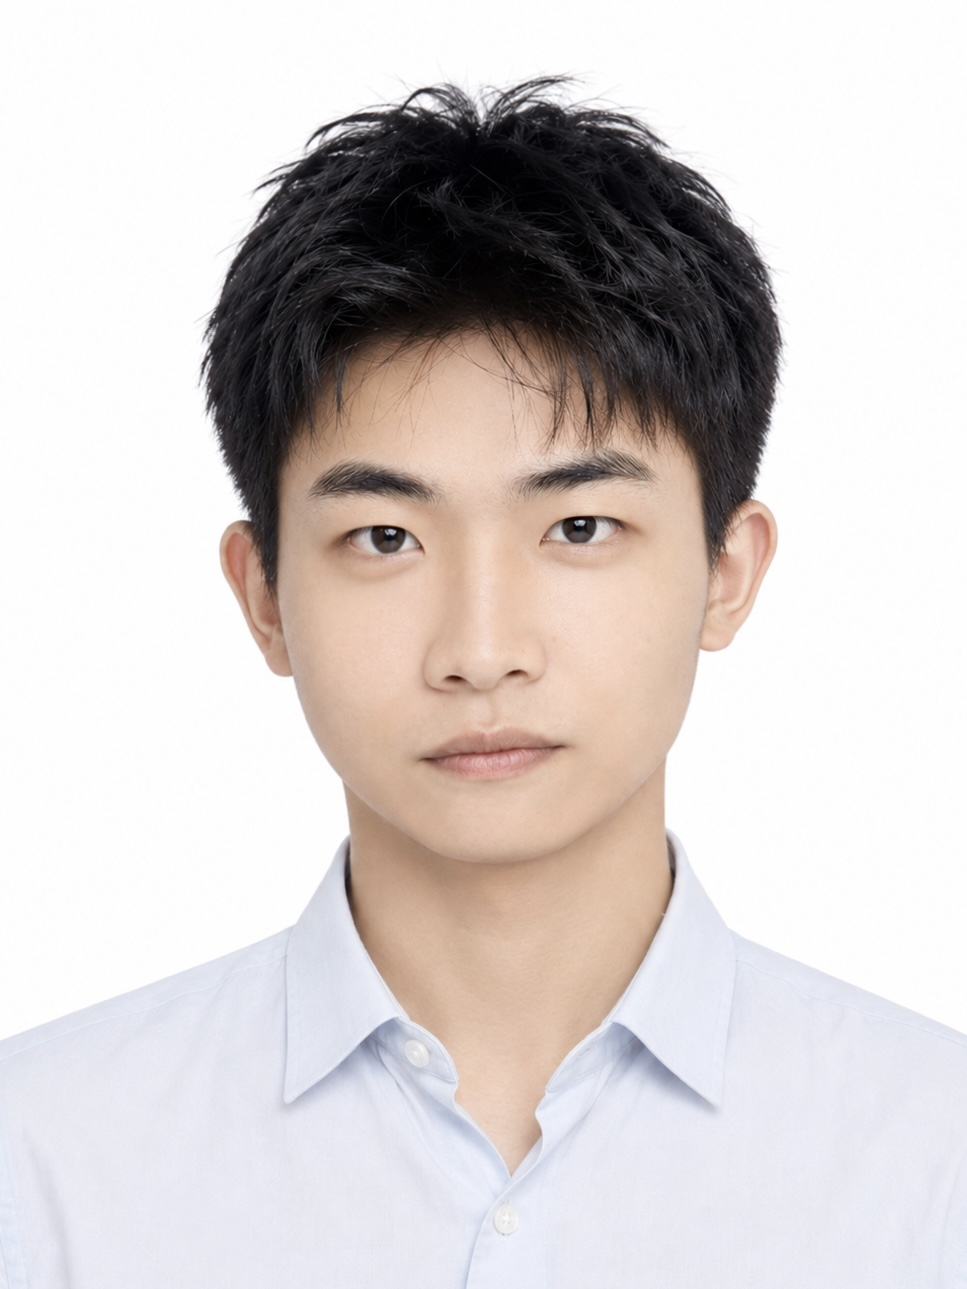
\includegraphics[width=2.05cm,height=2.65cm]{picture.jpg}}}%
\begin{center}
    {\fontsize{30}{34}\selectfont\bfseries Siyuan Mei}\\[5pt]
    {\large 计算机科学博士生 | 医学人工智能与计算机视觉}\\[4pt]
    \href{mailto:siyuan.mei@fau.de}{siyuan.mei@fau.de}
    \enspace | \enspace \href{https://siyuan-mei.github.io}{主页 (github.io)}
    \enspace | \enspace \href{https://scholar.google.com/citations?user=W_xPF2YAAAAJ\&hl}{Google Scholar}\\[3pt]
    \href{https://lme.tf.fau.de/persons/siyuan-mei/}{实验室主页}
    \enspace | \enspace \href{https://www.linkedin.com/in/siyuan-mei-409353247/}{LinkedIn}
    \enspace | \enspace \href{https://github.com/siyuan-mei}{GitHub}\\[4pt]
    FAU Erlangen-Nürnberg · Pattern Recognition Lab (LME) · Germany
\end{center}

\section{个人优势}
自驱力与目标感强，重视结果质量与执行效率。长期、系统的科研训练形成了快速学习、拆解复杂问题和持续交付的能力；以第一作者在 MICCAI、Pattern Recognition、Journal of Medical Imaging 等发表多项工作。具备清晰表达、课程教学、任务协调和跨机构协作经验，能够在研究推进与技术沟通之间高效衔接。具有创新与合作意识，曾作为主要执行者参与国际挑战并取得优异成绩。\par
\textbf{求职沟通：}欢迎围绕医学影像、计算机视觉、LLM 辅助软件工程及合适岗位展开交流，也感谢任何 job conversation。

\section{研究方向}
\textbf{医学人工智能：}医学图像重建、合成、分割与配准。\\
\textbf{计算机视觉：}扩散模型、流匹配、生成建模、表征学习与稠密预测。\\
\textbf{LLM 与智能体：}LLM 辅助软件工程、可复现实验工具与 agentic systems；持续系统学习 Stanford CS336、CS224N、CS234 等课程。

\section{教育经历}
\zhentry{FAU Erlangen-Nürnberg}{2023--2027（预计）}{计算机科学博士；导师：Andreas Maier 教授。}\\[3pt]
\zhentry{北京大学医学部 · AIMI Lab}{2026.05--2026.10}{访问学者；导师：Yixing Huang 教授。}\\[3pt]
\zhentry{FAU Erlangen-Nürnberg}{2020--2023}{医学工程硕士；毕业论文成绩 1.0；硕士阶段获两项 merit-based scholarship。}\\[3pt]
\zhentry{浙江科技大学}{2016--2020}{自动化专业工学学士；中德 2+3 项目（本科阶段在中德两地完成衔接培养）；优秀毕业生奖学金。}

\enlargethispage{2\baselineskip}
\section{专业经历}
\textbf{FAU Erlangen-Nürnberg, Pattern Recognition Lab} \hfill 2023--2027\\
\textit{计算机科学博士生；导师：Andreas Maier 教授}
\begin{itemize}
    \item 获 ERC 4D Nanoscope 项目全额资助，围绕骨微结构与重塑开展研究；开发 BigReg，用于高分辨率 X-ray 显微成像与光片荧光显微成像的高效多模态配准。
    \item 研究医学人工智能与计算机视觉，关注基础模型适配，以及 GAN、扩散模型和 flow matching 在医学图像生成中的应用。
    \item 讲授 Flat-panel CT Reconstruction；参与编写 Vibe Coding: Software Engineering with LLMs lecture slides，作为 Springer 图书配套教学资源。
    \item 代表成果包括 Pattern Recognition 第一作者论文、Journal of Medical Imaging Featured Paper，以及 MICCAI 2026 Oral Presentation。
\end{itemize}
\pagebreak
\textbf{北京大学医学部, AIMI Lab} \hfill 2026.05--2026.10\\
\textit{访问学者；导师：Yixing Huang 教授}\\
医学技术研究院 Artificial Intelligence for Medical Imaging Lab，240 Pathology Building, No. 38 Xueyuan Road, Haidian District, Beijing, China。
\begin{itemize}
    \item 参加 MICCAI BIC-MAC Challenge，训练多模态到 CT 的生成模型，用于 PET 衰减校正；验证集 CT 指标取得第一名。
    \item 系统了解 CT 临床端应用技术与成像流程；访问重庆 ICT Center，并参加清华大学 MISC 2026 会议。
\end{itemize}

\section{精选论文}
\begin{enumerate}
    \zhpub{Time Matters: Rethinking Diffusion and Flow Models in One-Step Medical Image Translation}{MICCAI 2026；第一作者；\zhlabel{Early Accept}；\zhlabel{Oral Presentation}}{\href{https://github.com/siyuan-mei/JiR\#citation}{Paper}；\href{https://github.com/siyuan-mei/JiR}{Code}}
    \zhpub{Detail Consistent Stage-Wise Distillation for Efficient 3D MRI Segmentation}{MICCAI 2026；合作作者；\zhlabel{Early Accept}；\zhlabel{Spotlight}}{\href{https://arxiv.org/abs/2605.26382}{Paper}；\href{https://github.com/ClinicaAlpha/DCD-3D-MedSeg}{Code}}
    \zhpub{Speech-Guided Multimodal Learning for Vocal Tract Segmentation in Real-Time MRI}{MICCAI 2026；合作作者；\zhlabel{Oral Presentation}}{\href{https://arxiv.org/abs/2605.18466}{Paper}}
    \zhpub{WING: A Window-Prior-Based Generative Network with Gated Inception for Cross-Modality CT Synthesis}{MICCAI MIART Workshop 2026；第一作者}{\href{https://arxiv.org/abs/2607.06234}{Paper}；\href{https://github.com/siyuan-mei/WING}{Code}}
    \zhpub{Vision Transformer Hook for Dense Predictions}{Pattern Recognition 179 (2026), 113818；第一作者}{\href{https://doi.org/10.1016/j.patcog.2026.113818}{Paper}；\href{https://github.com/siyuan-mei/ViT-Hook}{Code}}
    \zhpub{BigReg: An Efficient Registration Pipeline for High-Resolution X-Ray and Light-Sheet Fluorescence Microscopy}{Journal of Medical Imaging 12(5), 054004 (2025)；第一作者；\zhlabel{Featured Paper}}{\href{https://doi.org/10.1117/1.JMI.12.5.054004}{Paper}}
    \zhpub{Metal Inpainting in CBCT Projections Using Score-based Generative Model}{IEEE ISBI 2023；第一作者}{\href{https://doi.org/10.1109/ISBI53787.2023.10230638}{Paper}}
    \zhpub{TCCT: Trajectory-Conditioned CBCT Reconstruction for Sinusoidal Non-Circular Orbits with a Fourier Neural Operator}{MICCAI 2026；合作作者}{Poster}
    \zhpub{A Gradient-Based Approach to Fast and Accurate Head Motion Compensation in Cone-Beam CT}{IEEE Transactions on Medical Imaging (2024)；合作作者}{\href{https://doi.org/10.1109/TMI.2024.3474250}{Paper}}
\end{enumerate}

\section{荣誉、服务与资源}
\begin{itemize}
    \item MICCAI SynthRAD2025 Challenge：Task 2 第一名，Task 1 第四名。
    \item FAU 医学工程硕士阶段获两项 merit-based scholarship；获 ERC 4D Nanoscope 项目全额资助博士职位。
    \item 浙江科技大学优秀毕业生奖学金（2020）。
    \item 学术服务：Pattern Recognition 审稿人；MICCAI 审稿人；Journal of Medical Imaging Technical Editor。
    \item 开源与教学资源：\href{https://github.com/siyuan-mei/WING}{WING}、\href{https://github.com/siyuan-mei/JiR}{JiR}、\href{https://github.com/siyuan-mei/ViT-Hook}{ViT-Hook}；\href{https://github.com/PRLab-FAU/VibeCodingSlides}{Vibe Coding lecture slides}（Springer 图书配套资源）。
\end{itemize}

\section{语言与个人信息}
\textbf{语言能力：}中文（母语）｜英语（专业级）｜德语（C1 证书）。\\
\textbf{兴趣爱好：}健身、网球（Level 2.5）。\quad \textbf{MBTI（自评）：}ENTJ-A。

\end{document}
